\chapter{Authentication}
\label{ch:authentication}

\section{Identification vs. Authentication}
In the realm of computer security, it is crucial to distinguish between identification and authentication, as they serve different but complementary purposes.
\begin{itemize}
    \item \textbf{Identification} is the process by which an entity declares its identifier. For example, stating ``I am Stefano'' or typing a username such as \texttt{foobar} at a login prompt.
    \item \textbf{Authentication} is the process by which the entity provides a \textit{proof} that verifies its claimed identity. For example, providing an ID card, or entering the correct password associated with the username \texttt{foobar}.
\end{itemize}
Authentication serves as the absolute foundation for the subsequent \textit{authorization} phase, where the system decides what the authenticated entity is permitted to do.

\section{Characteristics of Authentication}
Authentication processes can be classified based on their directionality and the entities involved.

\subsection{Directionality}
\begin{itemize}
    \item \textbf{Unidirectional Authentication:} Only one entity proves its identity to the other. For instance, a user proving their identity to a server to log in. 
    \item \textbf{Bidirectional (Mutual) Authentication:} Both entities authenticate each other. For example, a user authenticates to a server, and the server simultaneously proves its identity to the user (often via digital certificates) to prevent man-in-the-middle attacks or phishing.
\end{itemize}

\subsection{Involved Entities}
Authentication can happen between any types of entities:
\begin{itemize}
    \item \textbf{Human to human:} For example, recognizing a person by their face or voice.
    \item \textbf{Human to computer:} A user typing a password into a laptop.
    \item \textbf{Computer to computer:} An API client authenticating to a backend server using a secret token or a certificate.
\end{itemize}

\section{The Three Factors of Authentication}
\begin{tcolorbox}[colback=blue!5!white,colframe=blue!75!black,title=Exam Insight]
Questions often ask you to analyze the security of custom authentication schemes (e.g., password recovery mechanisms, biometrics, hardware protocols). You should be ready to identify and highlight specific weaknesses---such as susceptibility to snooping, guessing, or cloning. Furthermore, you will be expected to systematically suggest appropriate improvements or multi-factor combinations to fix these flaws, directly linking each vulnerability to its corresponding countermeasure as discussed in class.
\end{tcolorbox}

Authentication mechanisms generally rely on one or more of three primary factors:
\begin{enumerate}
    \item \textbf{Something you \textit{know} (The ``to know'' factor):} A secret piece of information, such as a password, a PIN, or a secret handshake.
    \item \textbf{Something you \textit{have} (The ``to have'' factor):} A physical object, such as a door key, a smart card, a hardware token, or a smartphone.
    \item \textbf{Something you \textit{are} (The ``to be'' factor):} A physical or behavioral characteristic, such as a fingerprint, face geometry, or voice pattern (biometrics).
\end{enumerate}

In everyday human interactions, we primarily rely on the ``to be'' factor (recognizing faces), followed by ``to have'' (keys to a house), and rarely on ``to know'' (secret handshakes). In contrast, computer systems have historically relied heavily on the ``to know'' factor, followed by ``to have'', and only recently have begun adopting the ``to be'' factor widely. When a system combines two or more of these factors, it is known as \textbf{Multi-Factor Authentication (MFA)}.

\section{The ``To Know'' Factor: Passwords and PINs}
In this approach, the user must prove their identity by demonstrating knowledge of a secret.

\subsection{Advantages and Disadvantages}
The main \textbf{advantages} of passwords are their low cost, ease of deployment, and low technical barrier to entry. However, the \textbf{disadvantages} are significant. Secrets can be:
\begin{itemize}
    \item \textbf{Stolen or snooped:} Obtained via phishing, keyloggers, or simply looking over someone's shoulder (shoulder surfing) or finding sticky notes on monitors.
    \item \textbf{Guessed:} Attackers can guess common passwords (e.g., ``password123'') or passwords based on the user's personal information.
    \item \textbf{Cracked (enumerated):} Attackers can use brute-force or dictionary attacks against password databases to find the correct password.
\end{itemize}

\begin{tcolorbox}[colback=blue!5!white,colframe=blue!75!black,title=Exam Insight]
For exams, be prepared to analyze password and PIN entropy and formally calculate brute-forcing probabilities. You may be asked to compute the success probability of a brute-force attack given specific attacker constraints, such as an energy budget, computational limits, or a hash truncation bound. Ensure you are comfortable with probability formulas relating to search spaces and the impact of reduced entropy.
\end{tcolorbox}

\subsection{Countermeasures and the Cost of Security}
To mitigate these risks, systems enforce password policies (countermeasures):
\begin{itemize}
    \item Forcing passwords to change or expire frequently.
    \item Requiring long passwords with a rich character set (complexity).
    \item Ensuring passwords are not related to the user's personal data.
\end{itemize}

However, these countermeasures introduce usability \textit{costs}. Humans are not machines; we are inherently bad at keeping secrets and struggle to remember complex, randomly generated strings. When policies become too strict, users resort to insecure behaviors, such as writing passwords down on sticky notes or applying predictable transformations (e.g., changing \texttt{P@ssword1!} to \texttt{P@ssword2!}). Therefore, system designers must carefully estimate the most likely attacks and choose countermeasures that balance security with usability, often employing \textbf{password meters} to gently nudge users toward creating stronger passwords without imposing overly rigid rules.

\subsection{Password Managers}
To solve the problem of managing and remembering multiple complex passwords, \textbf{Password Managers} offer a solution. They rely on 1 identity, 1-2 authentication factors, and 1 trusted password vault.
\begin{itemize}
    \item \textbf{Pros:} Users no longer need to remember all their passwords, allowing for the generation of unique, highly robust passwords for every service. They also offer excellent usability via auto-fill and cross-device synchronization.
    \item \textbf{Cons:} They introduce a single point of trust and failure. If the master password is compromised, all accounts are exposed. Furthermore, they represent a larger attack surface, as they are complex software applications (and browser extensions) that may contain vulnerabilities.
\end{itemize}

\section{Secure Password Exchange and Storage}
Authentication involves sharing and storing secrets securely.

\subsection{Secure Password Exchange}
When transmitting a secret across a network, there is a risk of it being intercepted. To minimize this risk:
\begin{itemize}
    \item Use mutual authentication (e.g., TLS/HTTPS) to ensure the client is talking to the legitimate server.
    \item Use \textbf{Challenge-Response} or \textbf{Zero-Knowledge Proof} schemes.
\end{itemize}

\begin{figure}[h!]
    \centering
    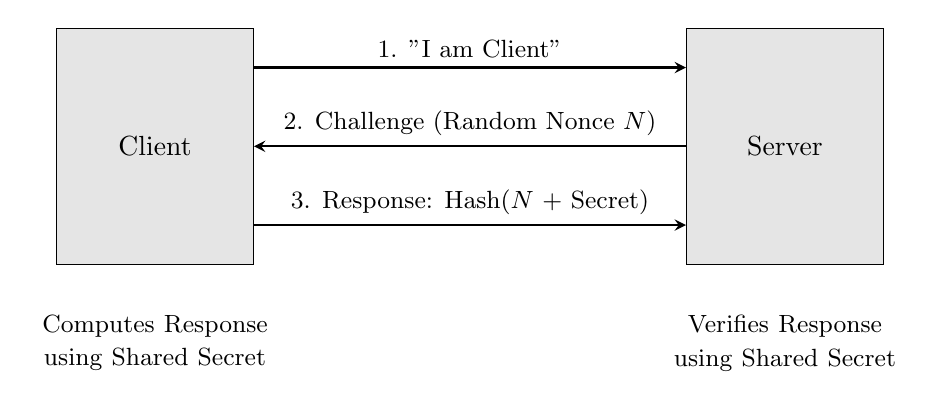
\begin{tikzpicture}[node distance=2cm, auto, >=stealth]
        % Nodes
        \node (client) [draw, rectangle, minimum height=3cm, minimum width=2.5cm, fill=gray!20] {Client};
        \node (server) [draw, rectangle, minimum height=3cm, minimum width=2.5cm, fill=gray!20, right of=client, node distance=8cm] {Server};
        
        % Arrows and text
        \draw[->, thick] ([yshift=1cm]client.east) -- node[above] {\small 1. "I am Client"} ([yshift=1cm]server.west);
        
        \draw[<-, thick] ([yshift=0cm]client.east) -- node[above] {\small 2. Challenge (Random Nonce $N$)} ([yshift=0cm]server.west);
        
        \draw[->, thick] ([yshift=-1cm]client.east) -- node[above] {\small 3. Response: Hash($N$ + Secret)} ([yshift=-1cm]server.west);
        
        % Annotations
        \node at (0, -2.5) [text width=3cm, align=center] {\small Computes Response\\ using Shared Secret};
        \node at (8, -2.5) [text width=3cm, align=center] {\small Verifies Response\\ using Shared Secret};
    \end{tikzpicture}
    \caption{A simple Challenge-Response authentication scheme. Replay attacks are mitigated because the nonce $N$ changes every session.}
    \label{fig:challenge_response}
\end{figure}

In a typical challenge-response scheme (Figure~\ref{fig:challenge_response}), the server sends a random challenge (e.g., a nonce) to the client. The client computes a cryptographic hash of the challenge combined with their secret password and sends it back. The server performs the same computation and verifies the result. Because the challenge changes every time, an attacker eavesdropping on the network cannot reuse the captured hash (\textbf{replay attack}).

\subsection{Secure Password Storage}
Operating systems and web servers must store user credentials. If an attacker compromises the server, the confidentiality of the password file is at risk. 
To minimize this risk:
\begin{itemize}
    \item \textbf{Never store passwords in cleartext.} Passwords must be protected cryptographically using one-way cryptographic hash functions.
    \item \textbf{Use Salting.} A random salt should be added to the password before hashing to defend against precomputed dictionary attacks (Rainbow Tables).
    \item Implement strict access control policies on the password file.
    \item Never disclose the actual secret in password-recovery schemes (e.g., sending the plaintext password via email is a severe security flaw).
\end{itemize}

\begin{tcolorbox}[colback=blue!5!white,colframe=blue!75!black,title=Exam Insight]
A typical exam scenario requires critically analyzing custom password recovery mechanisms. You must check if secrets are transmitted in plaintext, sent over unencrypted channels, or poorly stored in the backend database. You are expected to clearly highlight these vulnerabilities and propose concrete secure storage methods (such as salted hashes using strong one-way functions) and robust exchange protocols (like challenge-response or mutual authentication) as viable countermeasures to reduce the risk.
\end{tcolorbox}

\section{The ``To Have'' Factor: Tokens and Smart Cards}
Here, the user proves they possess a specific physical item.

\subsection{Advantages and Disadvantages}
\textbf{Advantages:} It leverages the human factor, as people are generally more protective of physical items (like keys or phones) than abstract passwords and will quickly notice if they are missing. It offers a good level of security at a relatively low cost.

\textbf{Disadvantages:} Physical tokens are harder to deploy logistically and can be lost or stolen. The primary countermeasure is to use them in combination with a second factor (e.g., a smart card that also requires a PIN).

\subsection{Classic and Modern Technologies}
\begin{itemize}
    \item \textbf{Static OTP Lists:} A cheap alternative where the user and host share a printed list of one-time passwords (e.g., a grid card).
    \item \textbf{Hardware One-Time Password (OTP) Generators:} A device holding a secret key synchronized with the host (via a counter or time). It generates a MAC (Message Authentication Code) that changes every 30-60 seconds.
    \item \textbf{Smart Cards:} Cards equipped with a CPU and non-volatile RAM holding a private key. They authenticate to the host via a challenge-response protocol (signing the challenge). The private key never leaves the tamper-proof device.
    \item \textbf{Modern TOTP Apps:} Software implementations of OTP generators (e.g., Google Authenticator). Unlike hardware tokens, these run on general-purpose smartphones, which introduces the risk of malware compromising the generated codes.
    \item \textbf{Secure Keys (e.g., YubiKeys):} Hardware-based devices that plug into a USB port or use NFC. They provide OTPs or use Public Key Cryptography (FIDO2/WebAuthn) for secure, phishing-resistant authentication.
\end{itemize}

A notable threat to mobile-based authentication (like SMS OTPs) is \textbf{SIM Swapping}, where an attacker uses social engineering against a telecom operator to port the victim's phone number to a SIM card controlled by the attacker.

\section{The ``To Be'' Factor: Biometrics}
Biometric authentication requires the user to prove they possess specific physical or behavioral characteristics. Examples include fingerprints, face geometry, hand geometry, retina/iris scans, voice analysis, DNA, and typing dynamics.

\subsection{Advantages and Disadvantages}
\textbf{Advantages:} High level of security and robustness. It requires no extra hardware for the user to carry around or remember.

\textbf{Disadvantages:} 
\begin{itemize}
    \item Hard to deploy (requires specialized sensors).
    \item \textbf{Probabilistic matching:} Unlike a password which is strictly right or wrong, biometrics rely on similarity thresholds, leading to \textit{false positives} (accepting an impostor) and \textit{false negatives} (rejecting the legitimate user).
    \item Invasive measurement and privacy sensitivity.
    \item Characteristics can change over time (e.g., due to injury or aging).
    \item Issues for users with physical disabilities.
    \item \textbf{Cloning:} Biometric traits can often be captured and replicated (e.g., lifting a fingerprint from a glass, or using high-resolution photos to fool facial recognition).
\end{itemize}

Because biometric traits cannot be easily changed once compromised (you cannot ``reset'' your fingerprint), systems must employ countermeasures like frequent re-measurement, liveness detection (to ensure a real human is present, not a photograph), and providing secure fallback authentication methods.

\section{Novel Factors and Single Sign-On}

\subsection{The ``Social'' Factor}
Experimental authentication methods involve proving \textit{who you know}. For example, Facebook has experimented with social authentication where a user, upon logging in from an unrecognized device, is asked to identify their friends from a selection of photos.

\subsection{Single Sign-On (SSO)}
To combat the fatigue of managing multiple passwords across countless websites, \textbf{Single Sign-On (SSO)} centralizes authentication. The solution involves one identity, 1-2 authentication factors, and one \textit{trusted host} (Identity Provider).

\begin{figure}[h!]
    \centering
    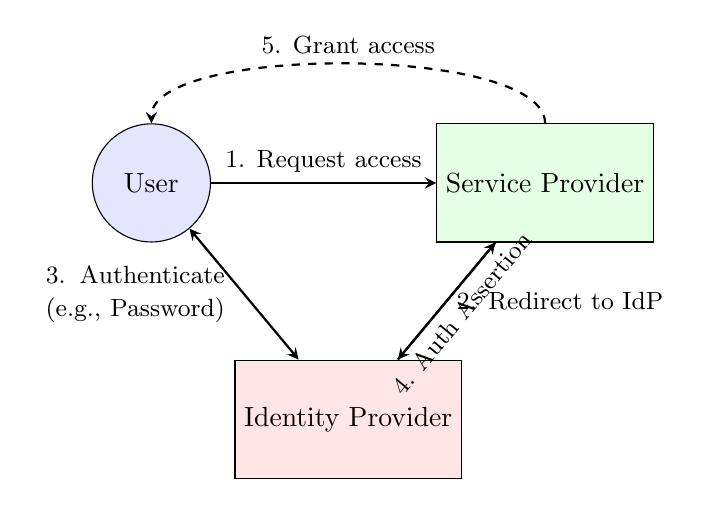
\begin{tikzpicture}[node distance=3cm, auto, >=stealth]
        \node (user) [draw, circle, minimum size=1.5cm, fill=blue!10] {User};
        \node (sp) [draw, rectangle, minimum height=1.5cm, minimum width=2.5cm, fill=green!10, right of=user, node distance=5cm] {Service Provider};
        \node (idp) [draw, rectangle, minimum height=1.5cm, minimum width=2.5cm, fill=red!10, below of=sp, node distance=3cm, xshift=-2.5cm] {Identity Provider};
        
        \draw[->, thick] (user) -- node[above] {\small 1. Request access} (sp);
        \draw[->, thick] (sp) -- node[right] {\small 2. Redirect to IdP} (idp);
        \draw[<->, thick] (user) -- node[left, text width=2.5cm, align=center] {\small 3. Authenticate\\ (e.g., Password)} (idp);
        \draw[->, thick] (idp) -- node[below, sloped] {\small 4. Auth Assertion} (sp);
        \draw[->, thick, dashed] (sp.north) .. controls +(up:1cm) and +(up:1cm) .. node[above] {\small 5. Grant access} (user.north);
    \end{tikzpicture}
    \caption{Simplified Single Sign-On (SSO) flow.}
    \label{fig:sso_flow}
\end{figure}

As shown in Figure~\ref{fig:sso_flow}, the user authenticates once with the trusted host. When accessing other services (Service Providers), those services ask the trusted host to verify the user's identity. Examples include Shibboleth (SAML) used in academia, and OAuth2/OpenID Connect used by major tech companies (e.g., ``Login with Google'').

\textbf{Challenges of SSO:}
\begin{itemize}
    \item It creates a \textbf{single point of trust}. If the identity provider is compromised, all linked services are compromised.
    \item The password reset scheme must be absolutely bulletproof (often relying on email as the root of trust).
    \item The cryptographic flows are complex for developers to implement correctly, often leading to subtle but critical vulnerabilities in the interactions between services.
\end{itemize}

\section{Passwordless Authentication: Passkeys}
The industry is moving toward \textbf{Passwordless Authentication} through the use of \textbf{Passkeys} (built on WebAuthn/FIDO2 standards). 
Instead of a shared secret (password), Passkeys use \textbf{Public Key Cryptography}. 
\begin{enumerate}
    \item \textbf{Registration:} The user's device generates a cryptographic key pair. The \textit{public key} is sent to the application's server. The \textit{private key} is securely stored on the user's device (e.g., in a secure enclave).
    \item \textbf{Login:} The server sends a cryptographic challenge. The user unlocks their private key locally using biometrics (FaceID, TouchID) or a device PIN. The device uses the private key to sign the challenge and returns it to the server, which verifies the signature using the stored public key.
\end{enumerate}
Because the private key never leaves the device, Passkeys are immune to phishing, server data breaches (the server only holds public keys), and credential stuffing attacks.

\section{Conclusions}
Identification, authentication, and authorization are distinct but inter-dependent concepts. There are three main types of authentication factors (to know, to have, to be), and for robust security, they should be used in combination (Multi-Factor Authentication). As traditional passwords increasingly show their limits and vulnerabilities, modern solutions like Password Managers, Single Sign-On, and particularly Passwordless schemes (Passkeys) are paving the way for a more secure and usable future, though they must be implemented and managed with care.

\section*{Chapter Summary}
This chapter explores the foundational concepts and mechanisms of authentication. It distinguishes authentication from identification, and details the Three Factors of Authentication: \textit{To Know} (passwords), \textit{To Have} (tokens), and \textit{To Be} (biometrics). The chapter also covers secure password handling, Single Sign-On (SSO), and modern Passwordless Authentication (Passkeys).

\begin{table}[h!]
    \centering
    \renewcommand{\arraystretch}{1.2}
    \begin{tabular}{|l|p{3.5cm}|p{4.2cm}|p{4.2cm}|}
        \hline
        \textbf{Factor} & \textbf{Examples} & \textbf{Advantages} & \textbf{Disadvantages} \\ \hline
        \textbf{To Know} & Passwords, PINs & Cheap, easy to deploy & Vulnerable to guessing/stealing, hard to remember \\ \hline
        \textbf{To Have} & Smart cards, OTP tokens, YubiKeys & Leverages human protection of physical items & Hard to deploy logistically, can be lost or stolen \\ \hline
        \textbf{To Be} & Fingerprints, Face geometry & High security, robust, no extra hardware & Probabilistic matching, privacy issues, cloning risk \\ \hline
    \end{tabular}
    \caption{Summary of the Three Authentication Factors}
    \label{tab:auth_factors}
\end{table}
